\documentclass[12pt,a4paper]{report}
\usepackage{a4wide}
\usepackage[portuguese,english]{babel}
\usepackage{graphics}
\usepackage{amsmath}
\usepackage{epsfig}
\usepackage[latin1]{inputenc}
\usepackage{doublespace}
\usepackage{fancyheadings}
\usepackage{longtable}
\usepackage{dropping}
\usepackage{url}
\usepackage{subfigure}
\usepackage[top=3cm,left=3cm,bottom=2cm,right=2cm]{geometry}


%\usepackage{apalike}
\newcommand{\figr}[1]{Figura~\ref{#1}}
\newcommand{\eqt}[1]{Eq.~(\ref{#1})}
\newcommand{\eqts}[2]{Eq.~(\ref{#1})~e~(\ref{#2})}
\newcommand{\eqtss}[3]{Eq.~(\ref{#1})~,~(\ref{#2})~e~(\ref{#3})}
\newcommand{\tab}[1]{Tabela~\ref{#1}}

%comandos para se definir cabe�alhos nas p�ginas da disserta��o
\pagestyle{fancyplain}
\lhead[\fancyplain{}{\thepage}]{\fancyplain{}{\small\leftmark}}
\rhead[\fancyplain{}{\small\rightmark}]{\fancyplain{}{\thepage}}
\cfoot{\fancyplain{\thepage}{}}

%package para reconhecimento de acentua��o em portugu�s
\usepackage[latin1]{inputenc}

%package para reconhecimento de portugu�s
\usepackage{babel}

%package para uso de verbatimtab
%\usepackage{moreverb}

%configura��o para numera��o de subsubse��es
\setcounter{secnumdepth}{3}

% Frases de efeito no in�cio de cada cap�tulo
\newcommand{\epigraph}[2]{%
  \vspace{1ex}%
  {\footnotesize%
   \begin{spacing}{1}
    \begin{flushright}%
      \begin{minipage}{.6\textwidth}%
        #1\\
      \end{minipage}\\
      \textit{#2}%
    \end{flushright}
    \end{spacing}}%
  \vspace{1ex}}



\begin{document}

%-----------------------------------
% CAPA EM PORTUGU�S
%-----------------------------------
\thispagestyle{empty}

\begin{spacing}{1.0}

\begin{center}
\begin{large}
\begin{huge}
CENTRO UNIVERSIT�RIO DA FEI\\[0.2 cm]
\end{huge}

\vspace {2 cm}


MAUR�CIO KENITI HIROTA\\[0.2 cm]

FABR�CIO LOPES DE SOUZA\\[0.2 cm]

IVAN SHIGUENORI MACHIDA\\[0.2 cm]

THIAGO MIZUTANI\\[0.2 cm]

Orientador: Prof. D.Sc. Paulo S�rgio Silva Rodrigues \\[0.2 cm]
\end{large}
\end{center}

\vspace {2 cm}

\begin{spacing}{1.5}
\begin{center}
\begin{huge}
{\bf MANUAL DE USO - M-FIT}
\end{huge}
\end{center}
\end{spacing}

\vspace {8 cm}

\begin{center}
\begin{large}
S�o Bernardo do Campo \\[0.2 cm]
2008
\end{large}
\end{center}

\end{spacing}
\newpage

%-----------------------------------
% CAPA DE APRESENTA��O EM PORTUGU�S
%-----------------------------------
\thispagestyle{empty}

\begin{spacing}{1.0}

\begin{center}
\begin{large}
\begin{huge}
CENTRO UNIVERSIT�RIO DA FEI\\[0.2 cm]
\end{huge}

\vspace {2 cm}

MAUR�CIO KENITI HIROTA\\[0.2 cm]

FABR�CIO LOPES DE SOUZA\\[0.2 cm]

IVAN SHIGUENORI MACHIDA\\[0.2 cm]

THIAGO MIZUTANI\\[0.2 cm]

Orientador: Prof. D.Sc. Paulo S�rgio Silva Rodrigues \\[0.2 cm]
\end{large}
\end{center}

\vspace {2 cm}

\begin{spacing}{1.5}
\begin{center}
\begin{huge}
{\bf MANUAL DE USO - M-FIT}

\end{huge}
\end{center}
\end{spacing}

\vspace {2 cm}

\begin{flushright}
\begin{minipage}[t]{8.5 cm}
Trabalho de Conclus�o de Curso, apresentado no Centro Universit�rio
da FEI, como parte dos requisitos necess�rios para obten��o do
t�tulo de Bacharel em Ci�ncias da Computa��o, orientado pelo
professor Prof. D.Sc. Paulo S�rgio Silva Rodrigues.
\end{minipage}
\end{flushright}

\vspace {2 cm}

\begin{center}
\begin{large}
S�o Bernardo do Campo \\[0.2 cm]
2008
\end{large}
\end{center}

\end{spacing}
\newpage


%-----------------------------------
% DOCUMENTA��O DO TRABALHO
%-----------------------------------

\renewcommand{\baselinestretch}{1.3}

\pagenumbering{roman}
%\setlength{\voffset}{0.0in}

%\begin{spacing}{1.0}
%\chapter*{Resumo \label{resumo}}

Na �rea de Editora��o de V�deos, uma das maiores demandas � a
detec��o de transi��o de tomadas, que � basicamente o corte de uma
tomada e o inicio de outra, o que � �til para diversas aplica��es,
como indexa��o, recupera��o, an�lise e edi��o de v�deos. Estas
transi��es podem ocorrer de diversas formas, tais como: zooms,
cortes, fades, dissolves. Este trabalho apresenta o M-FIT Motion
Finder Integration, um framework que possibilitar� o reconhecimento
autom�tico das transi��es de tomadas de cenas a partir de uma
determinada amostragem de imagens (frames de um filme) atrav�s do
uso de t�cnicas de Ritmo Visual e Morfologia Matem�tica, permitindo
que o ponto exato da transi��o seja obtido de uma maneira mais
pr�tica e r�pida. O M-FIT � uma ferramenta desenvolvida em linguagem
C, com utiliza��o de OpenCV (biblioteca para computa��o visual). Sua
interface � feita com a utiliza��o da ferramenta QT, tornando o
M-FIT um sistema com uma interface simples e de f�cil entendimento,
a qual ter� diversos atalhos para outras funcionalidades do sistema.

%\end{spacing}

%\begin{spacing}{1.0}
%\chapter*{\centering ABSTRACT \label{abstract}}

\hspace*{1.25cm}In the sector of Video Editorial, one of the biggest
demands is the detection of take transitions, which is basically the
cut of a take and the begin of another. This work have much
utilities in many applications, such as indexing, retrieval,
analysis and video editing. These transitions can occur in several
ways, such as: zooms, cuts, fades, and dissolve. This work presents
the M-FIT Motion Finder Integration, a framework that will let the
automatic detection of take transitions from a sample of images
(frames of a video) using techniques from Visual Rythim and
Mathematical Morphologie, allowing the exact point of transition is
obtained from a way practical and quickly. The M-FIT is a framework
developed in C language, with OpenCV (library to visual computing).
Your interface is made with QT, making M-FIT a system with a simple
interface and easy to understand, which will have many shortcuts to
another system features.

%\end{spacing}

\selectlanguage{portuguese}

\begin{spacing}{1.0}
\renewcommand{\contentsname}{Sum�rio}\tableofcontents
%\listoffigures
%\listoftables
\end{spacing}

\clearpage

\setcounter{page}{0} \pagenumbering{arabic}

% Aqui entram todos os t�picos
\begin{spacing}{1.5}

\section{CONHECENDO OS MENUS DO SISTEMA \label{introducao}}

\hspace*{1.25cm}Neste cap�tulo ser�o apresentados os menus do
sistema, com suas devidas funcionalidades.

\subsection{Arquivo \label{menu_arquivo}}

\hspace{1.25cm}Neste menu existem as seguintes op��es:

\begin{enumerate}

\item{\textbf{Cria��o de novo projeto:} Cria um novo projeto.}
\item{\textbf{Abrir Projeto:} Abre um projeto j� existente. S�o aceitos somente arquivos com a extens�o
MFIT}

\end{enumerate}

SIGAM ESSA LINHA DE RACIOC�NIO. Eu vo ajudar tamb�m mas n�o quero
saber de ficar fazendo tudo sozinho.

\section{FUNCIONALIDADES DO MFIT\label{introducao}}

\hspace*{1.25cm}Neste cap�tulo ser� explicado todas as funcionalidades do MFIT.

\subsection{Carregar um V�deo\label{carrega_video}}

\hspace{1.25cm}Nesta se��o detalharemos os passos necess�rios para se carregar um V�deo.

\begin{enumerate}

\item{Abra o MFIT (Figura \ref{img:mfit_aberto})}

\begin{figure}[h|top]
 \centering
 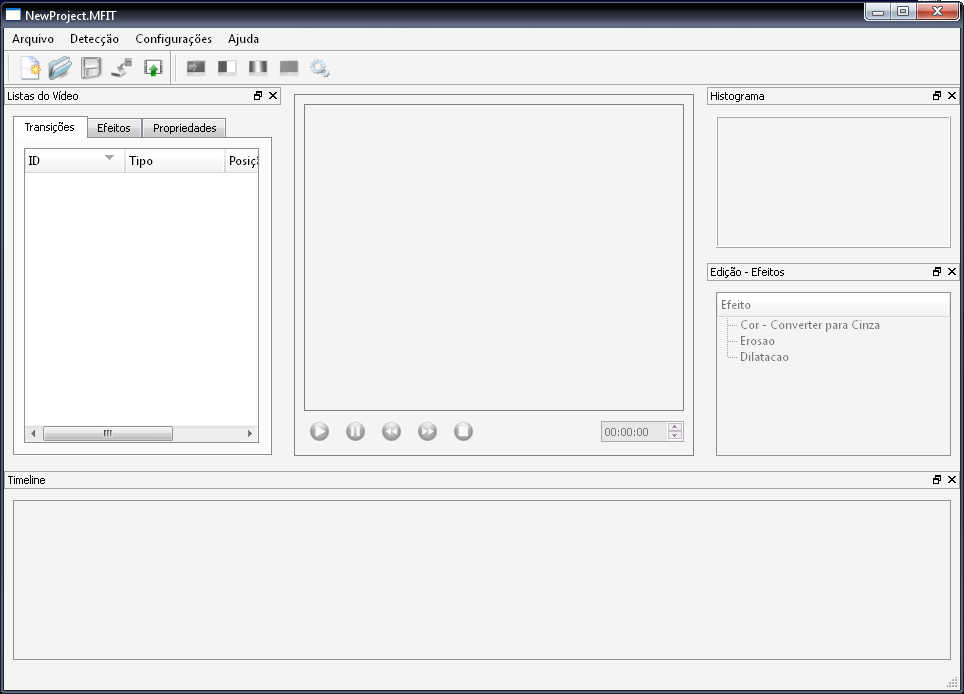
\includegraphics[width=0.7\linewidth]{imagens/mfit_aberto.png}
 \caption{MFIT Aberto sem V�deo carregado.}
 Fonte: Autor.
 \label{img:mfit_aberto}
\end{figure}

\item{Clique com o bot�o direito no menu "Arquivo", op��o "Carregar V�deo".
Se preferir, pressione as teclas Ctrl+Shif+O (Figura \ref{img:carregar2}). }

\begin{figure}[h|top]
 \centering
 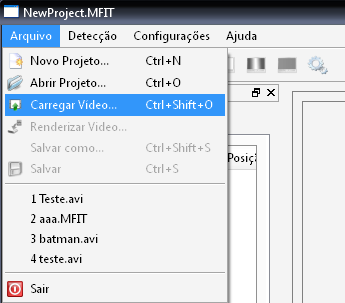
\includegraphics[width=0.7\linewidth]{imagens/carregar2.png}
 \caption{Menu "Arquivo", op��o "Carregar V�deo" .}
 Fonte: Autor.
 \label{img:carregar2}
\end{figure}

\item{Na janela que abrir�, selecione um V�deo v�lido (com extens�o .AVI) e de um duplo clique (Figura \ref{img:carregar3}). }

\begin{figure}[h|top]
 \centering
 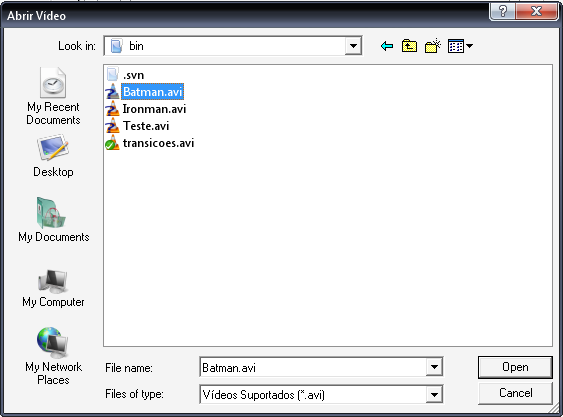
\includegraphics[width=0.7\linewidth]{imagens/carregar3.png}
 \caption{Selecionando um V�deo v�lido.}
 Fonte: Autor.
 \label{img:carregar3}
\end{figure}

\item{Ap�s alguns instantes o v�deo estar� aberto, e sua timeline estar� montada.
Note que uma janela se abrir�, questionando se o processo de detec��o de transi��es deve ser iniciado.
Por hora, clique em cancelar (Figura \ref{img:carregar4}). }

\begin{figure}[h|top]
 \centering
 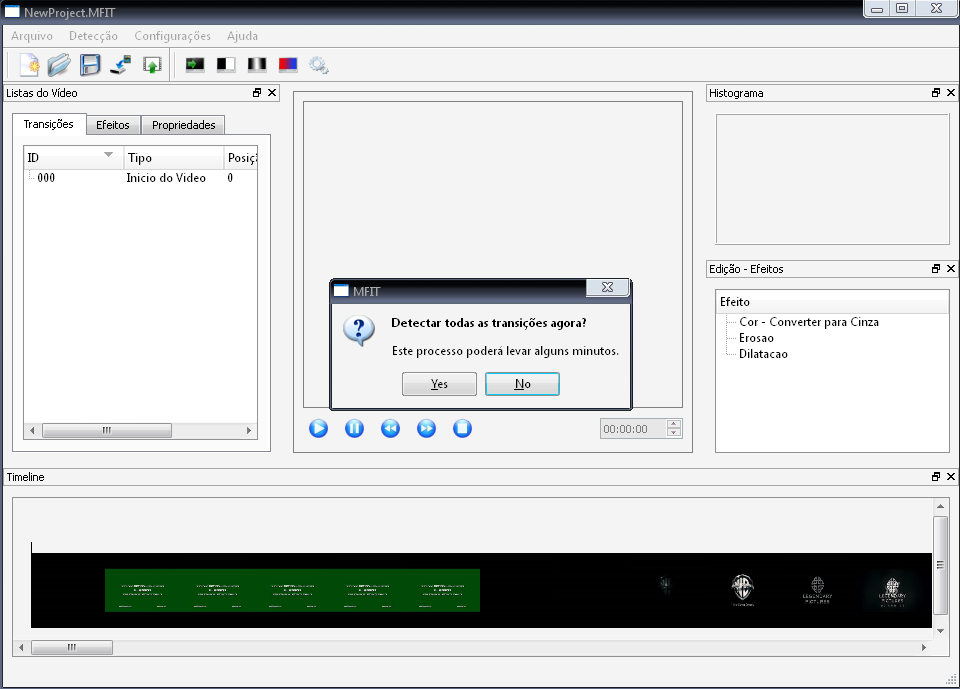
\includegraphics[width=0.7\linewidth]{imagens/carregar4.png}
 \caption{V�deo carregado e janela questionando o processo de detec��o.}
 Fonte: Autor.
 \label{img:carregar4}
\end{figure}

\item{Processo finalizado, o V�deo est� pronto para se efetuar todas as opera��es poss�veis (Figura \ref{img:carregar5}). }

\begin{figure}[h|top]
 \centering
 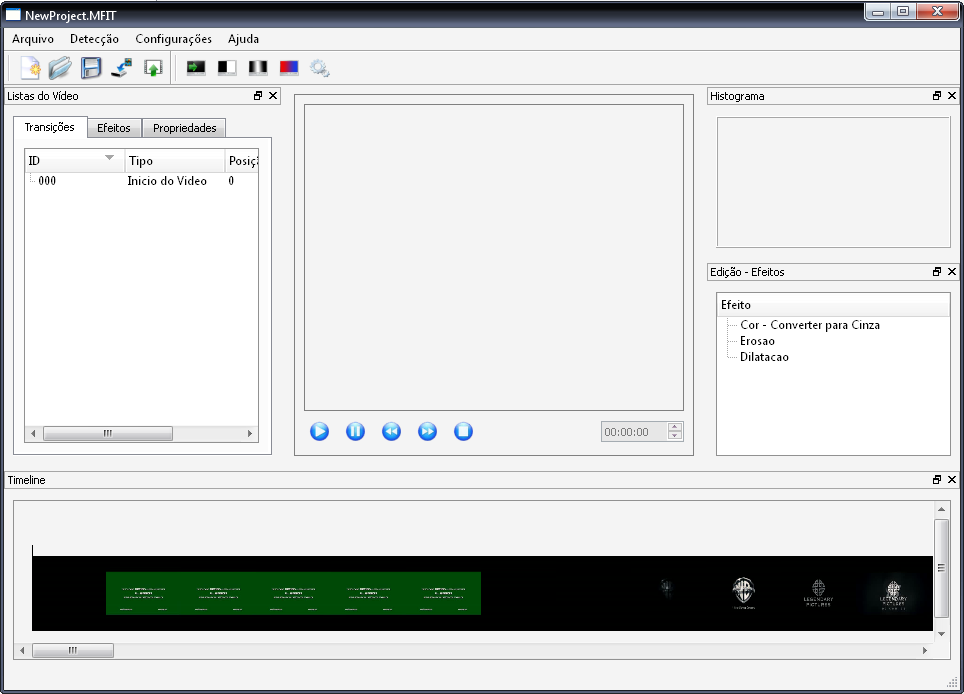
\includegraphics[width=0.7\linewidth]{imagens/carregar5.png}
 \caption{Fim do processo.}
 Fonte: Autor.
 \label{img:carregar5}
\end{figure}

\end{enumerate}

\subsection{Detec��o de transi��es\label{carrega_video}}

\hspace{1.25cm}Nesta se��o detalharemos os passos necess�rios para se detectar as transi��es de um V�deo.

\hspace{1.25cm}Para esta funcionalidade temos dois caminhos:

\begin{enumerate}
\item{� partir do carregamento do V�deo}

\subitem{ Ao chegar no passo 4 do processo de carregamento de V�deo (Se��o \ref{carrega_video}), existe a op��o de aceitar a detec��o de todas as transi��es.
Para isso, basta clicar em "OK" quando o sistema quiestionar sobre a detec��o. Com isso o processo de detec��o de todas as transi��es se iniciar�. ( Figura \ref{img:carregar4} )}

\item{Ap�s o carregamento do V�deo}

\subitem{ Ap�s realizar todos os passos do processo de carregamento do V�deo (Se��o \ref{carrega_video}), 
os bot�es de detec��o de transi��o estar�o habilitados. Escolha a detec��o que deseja e pressione o bot�o (Figura \ref{img:carregar5} )}

\item{ Ap�s escolher um dos passos acima, o sistema realizar� a detec��o de transi��es, com isso as transi��es ficar�o delimitadas
na Timeline, e a lista de transi��es ser� prenchida (Figura \ref{img:transicoes1}).}

\end{enumerate}

\begin{figure}[h|top]
 \centering
 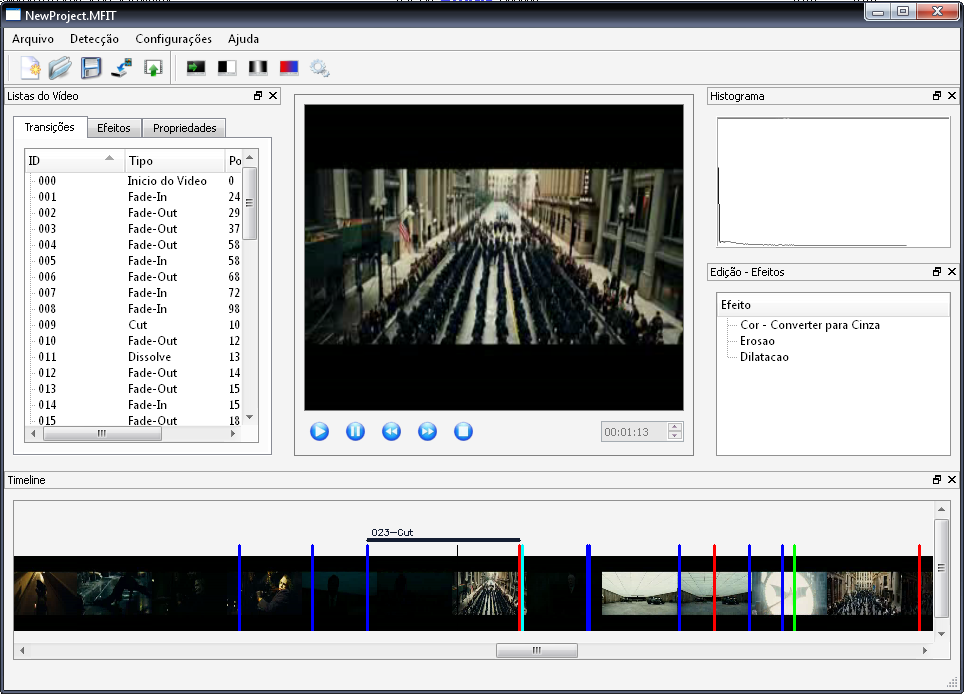
\includegraphics[width=0.8\linewidth]{imagens/transicoes1.png}
 \caption{Transi��es Detectadas.}
 Fonte: Autor.
 \label{img:transicoes1}
\end{figure}

\subsection{Aplica��o de Efeito\label{carrega_video}}

\hspace{1.25cm}Nesta se��o detalharemos os passos necess�rios para se aplicar um efeito no V�deo.
\hspace{1.25cm}Como pr�-requisito necessitamos de um V�deo carregado.

\begin{enumerate}

\item{Com o V�deo aberto, selecione um dos efeitos da lista de efeitos a direita (Figura \ref{img:efeitos1})}

\begin{figure}[h|top]
 \centering
 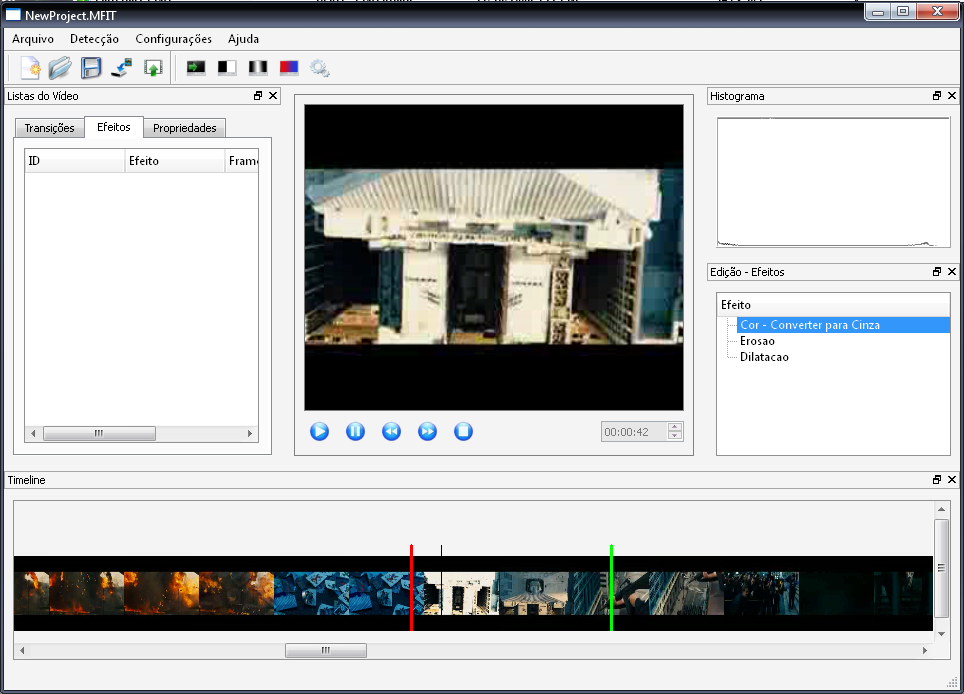
\includegraphics[width=0.7\linewidth]{imagens/efeitos1.png}
 \caption{Lista de Efeitos.}
 Fonte: Autor.
 \label{img:efeitos1}
\end{figure}

\item{Para aplicar o efeito, clique no efeito desejado e arraste para a posi��o o v�deo. Note que o sistema sinalizar�
	as transi��es onde este efeito ser� aplicado .(Figura \ref{img:efeitos2})}

\begin{figure}[h|top]
 \centering
 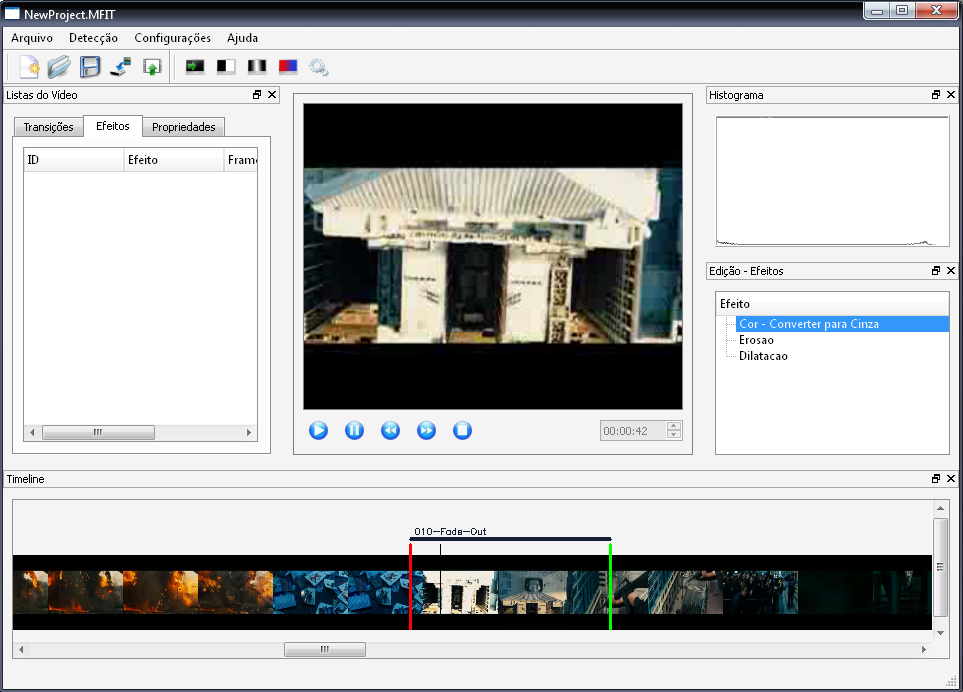
\includegraphics[width=0.7\linewidth]{imagens/efeitos2.png}
 \caption{Arrastando o efeito desejado.}
 Fonte: Autor.
 \label{img:efeitos2}
\end{figure}

\item{Caso o desejado seja aplicar em v�rias transi��es, no momento que estiver arrastando, segure a tecla CTRL (Figura \ref{img:efeitos3}).}

\begin{figure}[h|top]
 \centering
 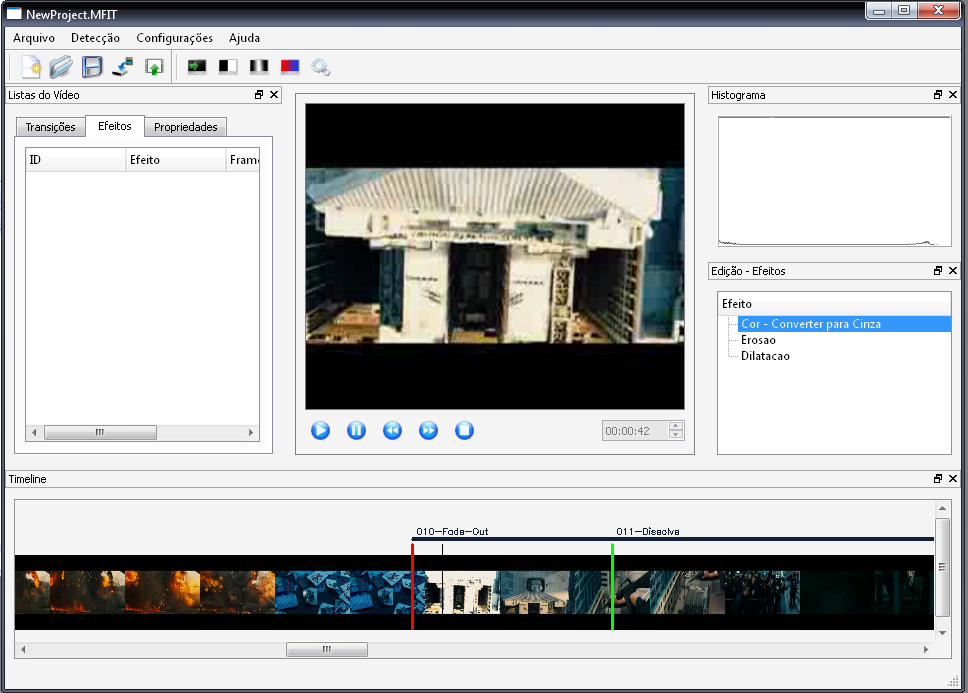
\includegraphics[width=0.7\linewidth]{imagens/efeitos3.png}
 \caption{Arrastando para m�ltiplas transi��es.}
 Fonte: Autor.
 \label{img:efeitos3}
\end{figure}

\item{Com isso o efeito vai ser aplicado no intervalo de transi��es desejados, note que a lista de efeitos conta agora com uma entrada, e a visualiza��o
	do v�deo j� contem o efeito aplicado (Figura \ref{img:efeitos4})}

\begin{figure}[h|top]
 \centering
 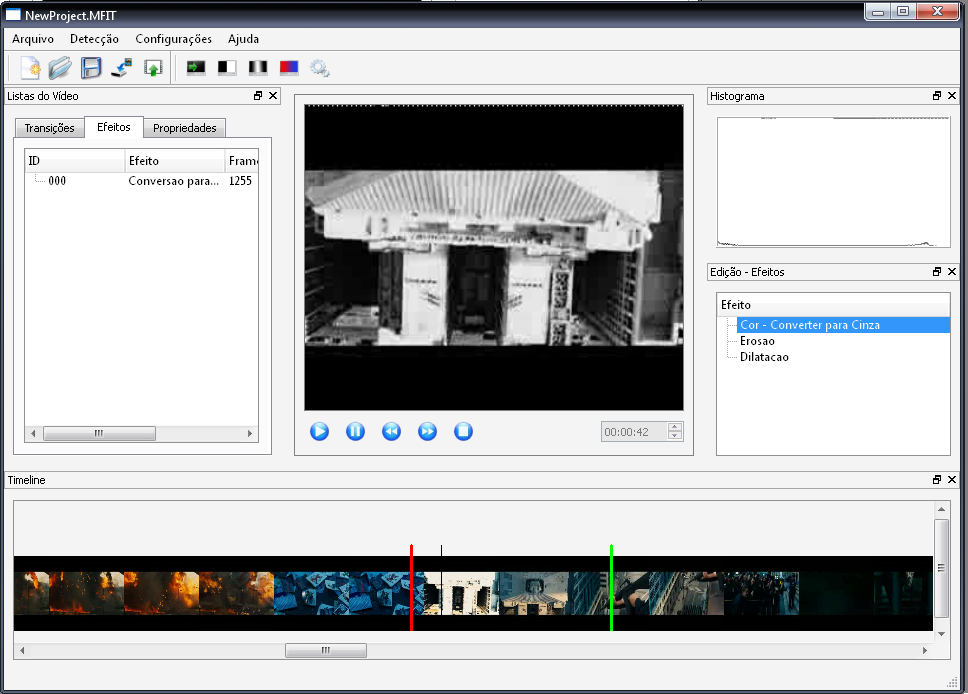
\includegraphics[width=0.7\linewidth]{imagens/efeitos4.png}
 \caption{Efeito aplicado.}
 Fonte: Autor.
 \label{img:efeitos4}
\end{figure}

\end{enumerate}


\end{spacing}

\appendix

%\include{apendice}

%Bibliografia
\begin{spacing}{1.0}
\bibliographystyle{apalike}
%\bibliographystyle{abbrv}
\bibliography{referencias}
\end{spacing}

\end{document}
